\cleartooddpage[\thispagestyle{empty}]
\chapter{Datatype Conversion and File Utilities}\label{io}
\moduleinfo{io}
The ``io'' module provides data import, export and datatype conversion. 
Four datatypes are supported by the ``io'' module: space-delimited values (txt), comma-separated values (csv), nested Tcl lists, or matrices (mat), and Tda tables (tbl). 
\clearpage
\section{File Utilities}
The commands \cmdlink{readFile}, \cmdlink{writeFile}, and \cmdlink{appendFile} simplify reading and writing of files in Tcl. Syntax is inspired from similar commands in the Tcllib fileutil package.
\begin{syntax}
\command{readFile} <\$option \$value ...> <-newline> \$filename
\end{syntax}
\begin{args}
\$option \$value ... & File configuration options, see Tcl \textit{fconfigure} command. \\
-nonewline & Option to read the final newline if it exists. \\
\$filename & File to read data from.
\end{args}
\begin{syntax}
\command{writeFile} <\$option \$value ...> <-nonewline> \$filename \$data
\end{syntax}
\begin{args}
\$option \$value ... & File configuration options, see Tcl \textit{fconfigure} command. \\
-nonewline & Option to not write a final newline. \\
\$filename & File to write data to. \\
\$data & Data to write to file.
\end{args}
\begin{syntax}
\command{appendFile} <\$option \$value ...> <-nonewline> \$filename \$data
\end{syntax}
\begin{args}
\$option \$value ... & File configuration options, see Tcl \textit{fconfigure} command. \\
-nonewline & Option to not write a final newline. \\
\$filename & File to append data to. \\
\$data & Data to append to file.
\end{args}
\begin{example}[label=ex:import_export]{File import/export}
\begin{lstlisting}
# Export data to file (creates or overwrites the file)
writeFile example.txt "hello world"
appendFile example.txt "goodbye moon"
# Import the contents of the file (requires that the file exists)
puts [readFile example.txt]
\end{lstlisting}
\tcblower
\begin{lstlisting}
hello world
goodbye moon
\end{lstlisting}
\end{example}
\clearpage
\section{Data Conversion}
The ``io'' module provides conversion utilities for different datatypes.  The intermediate format for Tda data conversion is matrix, or \textbf{mat}. 
\subsection{Matrix (mat)}
The matrix (\textbf{mat}) datatype is a nested Tcl list, where each list element represents a row vector of equal length. The ``io'' module is based around the \textbf{mat} datatype. An example of a matrix with headers is shown below. 
\begin{example}{Example Data (\textbf{mat}):}
\begin{lstlisting}
{step disp force} {1 0.02 4.5} {2 0.03 4.8} {3 0.07 12.6}
\end{lstlisting}
\end{example}
This format can be converted from and to all other formats, as is illustrated in the diagram below, with ``a'' \& ``b'' acting as placeholders for all other datatypes.
\begin{center}
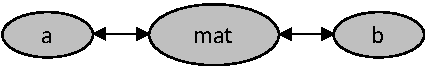
\includegraphics{dataconversion}
\end{center}
This way, each new datatype only requires the addition of two new conversion commands: one to \textbf{mat} and one from \textbf{mat}.
\clearpage
\subsection{Space-Delimited Text (txt)}
The space-delimited text (\textbf{txt}) datatype is simply space-delimited values, where new lines separate rows. Escaping of spaces and newlines is consistent with Tcl rules for valid lists. This is the datatype outputted by OpenSees recorders with the -file option. An example of the same data from the matrix example in \textbf{txt} format is shown below.
\begin{example}{Example Data (\textbf{txt}):}
\begin{lstlisting}
step disp force
1 0.02 4.5
2 0.03 4.8
3 0.07 12.6
\end{lstlisting}
\end{example}
To convert between \textbf{mat} \& \textbf{txt}, use the commands \cmdlink{mat2txt} \& \cmdlink{txt2mat}. 
\begin{syntax}
\command{mat2txt} \$mat <\$includeHeaders> <\$includeRownames>
\end{syntax}
\begin{args}
\$mat & Tcl matrix \\
\$includeHeaders & Boolean, whether to include first row of the matrix. Default true \\
\$includeRownames & Boolean, whether to include first column of the matrix. Default true
\end{args}
\begin{syntax}
\command{txt2mat} \$txt <\$includeHeaders> <\$includeRownames>
\end{syntax}
\begin{args}
\$txt & Space \& newline-delimited table \\
\$includeHeaders & Boolean, whether to include first row of the text data. Default true \\
\$includeRownames & Boolean, whether to include first column of the text data. Default true
\end{args}
\clearpage
\subsection{Comma-Separated Values (csv)}
The comma-separated values (\textbf{csv}) datatype is comma delimited values, where new lines separate rows. Commas and newlines are escaped with quotes, and quotes are escaped with double-quotes. This datatype is commonly used in post-processing and plotting programs, such as MS Excel. An example of the same data from the matrix example in \textbf{csv} format is shown below.
\begin{example}{Example Data (\textbf{csv}):}
\begin{lstlisting}
step,disp,force
1,0.02,4.5
2 0.03,4.8
3,0.07,12.6
\end{lstlisting}
\end{example}
To convert between \textbf{mat} \& \textbf{csv}, use the commands \cmdlink{mat2csv} \& \cmdlink{csv2mat}. 
\begin{syntax}
\command{mat2csv} \$mat <\$includeHeaders> <\$includeRownames>
\end{syntax}
\begin{args}
\$mat & Matrix \\
\$includeHeaders & Boolean, whether to include first row of the matrix. Default true \\
\$includeRownames & Boolean, whether to include first column of the matrix. Default true
\end{args}
\begin{syntax}
\command{csv2mat} \$csv <\$includeHeaders> <\$includeRownames>
\end{syntax}
\begin{args}
\$csv & Comma-separated values (with escaped commas, newlines, and quotes) \\
\$includeHeaders & Boolean, whether to include headers from CSV data. Default true \\
\$includeRownames & Boolean, whether the CSV data has rownames. Default true
\end{args}
\clearpage
\subsection{Table (tbl)}
The table (\textbf{tbl}) datatype represents tabular data with row and column names, and are created and manipulated with the table module. 
If headers or row names are not included when converting to tabular data, default keys and fields will be generated, with keys starting at 0 and fields starting at ``A''.
To convert between ``mat'' \& ``tbl'', use the commands \cmdlink{mat2tbl} \& \cmdlink{tbl2mat}.
\begin{syntax}
\command{mat2tbl} \$mat <\$includeHeaders> <\$includeRownames>
\end{syntax}
\begin{args}
\$mat & Matrix \\
\$includeHeaders & Boolean, whether to include first row of the matrix. Default true \\
\$includeRownames & Boolean, whether to include first column of the matrix. Default true
\end{args}
\begin{syntax}
\command{tbl2mat} \$tableObj <\$includeHeaders> <\$includeRownames>
\end{syntax}
\begin{args}
\$tableObj & Table object name \\
\$includeHeaders & Boolean, whether to include table fields as headers. Default true \\
\$includeRownames & Boolean, whether to include table keys as the first column. Default true
\end{args}
\clearpage
\subsection{Conversion Shortcuts}
Using the \textbf{mat} datatype as the intermediate datatype, data can be converted to and from any datatype, as is shown in the example below. 
\begin{example}{Example Code (using \textbf{mat} as intermediate):}
\begin{lstlisting}
set txt {step disp force
1 0.02 4.5
2 0.03 4.8
3 0.07 12.6}
set mat [txt2mat $txt]
set csv [mat2csv $mat]
puts $csv
\end{lstlisting}
\tcblower
\begin{lstlisting}
step,disp,force
1,0.02,4.5
2,0.03,4.8
3,0.07,12.6
\end{lstlisting}
\end{example}
For data conversions that use matrix as an intermediate format, shortcut commands are provided, illustrated in the table below. The optional arguments \texttt{\$includeHeaders} \& \texttt{\$includeRownames} are the same for the shortcut conversion commands.
\begin{center}
\begin{tabular}{|r|c|c|c|}
\hline
& \textbf{txt} & \textbf{csv} & \textbf{tbl} \\
\hline
\textbf{txt} & \cellcolor{gray} & \command{txt2csv} & \command{txt2tbl} \\
\hline
\textbf{csv} & \command{csv2txt} &  \cellcolor{gray} & \command{csv2tbl} \\
\hline
\textbf{tbl} & \command{tbl2txt} & \command{tbl2csv} & \cellcolor{gray} \\
\hline
\end{tabular}
\end{center}
One application of a shortcut conversion is bulk conversion of all recorder output files to \textbf{csv}.
\begin{example}{Example Code (convert .out files to .csv):}
\begin{lstlisting}
foreach filename [glob *.out] {
    writeFile [file rootname $filename].csv [txt2csv [readFile $filename]]
}
\end{lstlisting}
\end{example}
\section{Data Import and Export Shortcuts}
In addition to the fundamental file utilities and data conversion commands, the ``data'' module also provides some shortcut commands for common data import and export workflows.
\subsection{Matrix Import and Export}
The commands \cmdlink{readMatrix} and \cmdlink{writeMatrix} read/write a matrix from/to a file, converting from/to \textbf{csv} if the extension is .csv, and converting from/to \textbf{txt} otherwise.
Except for the input argument \texttt{\$matrix}, the input arguments are identical to \cmdlink{readFile} and \cmdlink{writeFile}.
\begin{syntax}
\command{readMatrix} <\$option \$value ...> <-newline> \$filename
\end{syntax}
\begin{syntax}
\command{writeMatrix} <\$option \$value ...> <-nonewline> \$filename \$matrix
\end{syntax}
\begin{args}
\$matrix & Matrix to convert and write to file.
\end{args}
\subsection{Table Import and Export}
The commands \cmdlink{readTable} and \cmdlink{writeTable} read/write a table from/to a file, converting from/to \textbf{csv} if the extension is .csv, and converting from/to \textbf{txt} otherwise.
Except for the input argument \texttt{\$table}, the input arguments are identical to \cmdlink{readFile} and \cmdlink{writeFile}.
\begin{syntax}
\command{readTable} <\$option \$value ...> <-newline> \$filename
\end{syntax}
\begin{syntax}
\command{writeTable} <\$option \$value ...> <-nonewline> \$filename \$table
\end{syntax}
\begin{args}
\$table & Table to convert and write to file.
\end{args}
\clearpage





